% Lernblatt Terme – gebaut aus der Aufgabenbank (bank/terme) nach Prompt
% v5.1, Vorbild Muster 4 (bau/terme/muster-2026-10-01/muster4.tex).
% Blattfolge der Mappe: Einheit 2, 3, 4, 1 → hier 1 Zusammenfassen,
% 2 Klammern auflösen, 3 Ausklammern, 4 Terme aufstellen und berechnen;
% Blatt 0 davor, „Zum Schluss“ und Lösungen dahinter.
% Quelle je Teilaufgabe im Kommentar davor: % <id> = aus der Bank (Auftrag im
% Titel der Nummer), % GEÄNDERT <id> = Form oder Zahlen geändert,
% % NEU = nicht in der Bank. % pruef: … = Rechenprobe (pruef.py).
\documentclass[11pt]{article}
\usepackage{mathblatt}
\usepackage{multicol}
\usepackage{lastpage}
% Kopf: nur das Thema; Fuß: „Seite n von m“
\pagestyle{fancy}\fancyhf{}\renewcommand{\headrulewidth}{0pt}
\setlength{\headheight}{14pt}
\fancyhead[L]{\small Terme}
\fancyfoot[C]{\small Seite \thepage\ von \pageref{LastPage}}
\raggedright
\makeatletter
% ---------------------------------------------------------------- Satz
\newcommand{\vorgerechnet}[1]{\textcolor{gray!70}{#1}}
\newcommand{\einheit}[2]{\par\Needspace*{0.33\textheight}\addvspace{16pt}%
  \noindent{\Large\bfseries\ifblank{#1}{}{#1\hspace{0.6em}}#2}\par\nobreak\vspace{2pt}%
  \gappto\mblsg{\lsgeinheit{\ifblank{#1}{}{#1\ }#2}}}
\newsavebox{\nrbox}\newlength{\nrhoehe}
\newcommand{\nrtitel}[1]{\noindent\hangindent1.6em\hangafter1%
  \makebox[1.6em][l]{\textbf{\theaufgabe.}}#1\par\vspace{1pt}}
\newenvironment{nr}[2][]{\refstepcounter{aufgabe}\setcounter{teil}{0}%
  \def\nrart{#1}%
  \ifx\nrart\@empty
    \begin{lrbox}{\nrbox}\begin{minipage}[t]{\linewidth}\raggedright
    \setlength{\parskip}{0pt}\nrtitel{#2}%
  \else
    \par\addvspace{11pt}\Needspace*{8\baselineskip}\nrtitel{#2}%
  \fi}%
 {\ifx\nrart\@empty
    \end{minipage}\end{lrbox}%
    \setlength{\nrhoehe}{\dimexpr\ht\nrbox+\dp\nrbox\relax}%
    \par\addvspace{11pt}\Needspace*{\nrhoehe}\noindent\usebox{\nrbox}\par
  \else\par\fi}
\newcommand{\teilmarke}{\stepcounter{teil}\makebox[1.6em][r]{\alph{teil})\hspace{0.35em}}}
\newcommand{\marke}[1]{\ifblank{#1}{}{\hfill{\footnotesize #1}}}
\newlength{\feldbreite}\setlength{\feldbreite}{4.5cm}
\newcommand{\antwort}{\underline{\hspace{\feldbreite}}}
\newcommand{\zeilenluft}{\par\nobreak\vskip 12pt plus 1pt\relax}
\newcommand{\zeilenluftb}{\par\vskip 12pt plus 1pt\relax}
\newlength{\kw}\newlength{\kwmax}
\newcounter{kzahl}\newcounter{kzeile}
\newcommand{\kliste}{}
\newcommand{\kmerke}[2]{\settowidth{\kw}{#1}%
  \ifdim\kw>\kwmax\global\kwmax=\kw\fi\stepcounter{kzahl}\gappto\kliste{#2}}
\newcommand{\kstart}[1]{\global\kwmax=0pt\setcounter{kzahl}{0}\setcounter{kzeile}{0}%
  \gdef\kliste{}\setlength{\feldbreite}{#1}}
\newcommand{\kende}{\par\vspace{3pt}\kliste\par}
\newcommand{\kettezeile}[1]{\stepcounter{kzeile}%
  \ifnum\value{kzeile}>1
    \ifnum\value{kzeile}<4 \zeilenluft
    \else\ifnum\numexpr\value{kzahl}-\value{kzeile}\relax<2 \zeilenluft
    \else\zeilenluftb\fi\fi
  \fi
  \noindent#1\par}
\newenvironment{kette}[1][4.5cm]{\kstart{#1}}{\kende}
\newcommand{\termspalte}[1]{\makebox[\kwmax][l]{$#1 =$}\hspace{0.6em}}
\NewDocumentCommand{\rk}{O{} m m}{\kmerke{$#2 =$}{\kettezeile{\teilmarke\lsgm{#3}%
  \termspalte{#2}\antwort\marke{#1}}}}
\newcommand{\rkv}[2]{\kmerke{$#1 =$}{\kettezeile{\teilmarke\termspalte{#1}%
  \vorgerechnet{$#2$}}}}
\newenvironment{werte}[1][2.8cm]{\kstart{#1}}{\kende}
\newcommand{\wertkopf}[2]{$#1$\hspace{0.8em}für $#2$:}
\NewDocumentCommand{\rw}{O{} m m m}{\kmerke{\wertkopf{#2}{#3}}{\kettezeile{\teilmarke\lsgm{#4}%
  \makebox[\kwmax][l]{\wertkopf{#2}{#3}}\hspace{0.6em}\antwort\marke{#1}}}}
\newcommand{\rwv}[3]{\kmerke{\wertkopf{#1}{#2}}{\kettezeile{\teilmarke
  \makebox[\kwmax][l]{\wertkopf{#1}{#2}}\hspace{0.6em}\vorgerechnet{$#3$}}}}
\NewDocumentCommand{\rt}{O{} m m}{\par\vspace{7pt}\noindent\hangindent1.6em\hangafter1
  \teilmarke\lsgt{#3}#2\nobreak\hspace{0.6em}\underline{\hspace{4cm}}\marke{#1}\par}
\newlength{\kennbreite}\setlength{\kennbreite}{1.6cm}
\NewDocumentCommand{\rtx}{O{} m m}{\par\vspace{7pt}\noindent
  \ifblank{#1}{\parbox[t]{\linewidth}{\raggedright\hangindent1.6em\hangafter1
   \teilmarke\lsgt{#3}#2}}%
  {\parbox[t]{\dimexpr\linewidth-\kennbreite\relax}{\raggedright\hangindent1.6em\hangafter1
   \teilmarke\lsgt{#3}#2}\parbox[t]{\kennbreite}{\raggedleft\footnotesize #1}}\par}
\NewDocumentCommand{\rs}{O{} m m}{\par\vspace{9pt}\noindent
  \teilmarke\lsgt{#3}%
  \ifblank{#1}{\parbox[t]{\dimexpr\linewidth-1.6em\relax}{\raggedright #2}}%
   {\parbox[t]{\dimexpr\linewidth-1.6em-\kennbreite\relax}{\raggedright #2}%
    \parbox[t]{\kennbreite}{\raggedleft\footnotesize #1}}\par\raum}
\newcommand{\raum}{\par\nobreak\vspace{7mm}\noindent\hspace*{1.6em}%
  \rule{0.5\textwidth}{0.4pt}\par\nobreak\vspace{7mm}\noindent\hspace*{1.6em}%
  \rule{0.5\textwidth}{0.4pt}\par}
\newcommand{\kreuzzeile}[1]{\par\vspace{6pt}\noindent\hspace*{1.6em}#1\par}
\renewcommand{\kreuz}[1]{$\square$\,#1\hspace{2.2em}}
\newcommand{\figurfelder}[2]{\par\vspace{6pt}\noindent\hspace*{1.6em}%
  $\vcenter{\hbox{#1}}$\hspace{1.5em}\begin{tabular}[c]{@{}l@{\hspace{0.5em}}l@{}}#2\end{tabular}\par}
% Merkkasten: schmaler Rahmen, je Zeile ein Fall (Stichwort fett, Beispiel,
% Ergebnis fett), zuletzt „Wichtig:“
\newcommand{\merk}[1]{\par\nobreak\vspace{5pt}\noindent
  \fcolorbox{black!60}{white}{\parbox{\dimexpr\linewidth-2\fboxsep-2\fboxrule\relax}{%
  \raggedright\setlength{\parskip}{1.5pt}#1}}\par\vspace{2pt}}
\newcommand{\mz}[2]{\textbf{#1} #2\par}
% ---------------------------------------------------------------- Lösungen
\newcommand{\mblsg}{}
\newcommand{\lsgm}[1]{\lsgt{$#1$}}
\newcommand{\lsgextra}{}
\newcommand{\lsgt}[1]{\xappto\mblsg{\noexpand\lz{\theaufgabe}{\alph{teil}}}%
  \xappto\mblsg{{\unexpanded{#1}\unexpanded\expandafter{\lsgextra}}}%
  \gdef\lsgextra{}}
\newcommand{\falsch}[1]{\gdef\lsgextra{\quad{\footnotesize falsch $\rightarrow$ Nr.~#1}}}
\newcommand{\falschk}[1]{\gappto\kliste{\falsch{#1}}}
\newcommand{\lzletzte}{0}
\newcommand{\lz}[3]{\par\noindent\hangindent3.4em\hangafter1
  \ifnum#1=\lzletzte\relax\makebox[1.8em][l]{}\else\makebox[1.8em][l]{\textbf{#1}}\fi
  \gdef\lzletzte{#1}%
  \makebox[1.6em][l]{\ifx&#2&\else#2)\fi}#3\par}
\newcommand{\lsgeinheit}[1]{\par\addvspace{4pt}\noindent{\bfseries #1}\par}
\makeatother

\begin{document}
\setlength{\parskip}{0pt}

% =================================================================== Blatt 0
\einheit{}{Das kennst du schon}
\noindent
\begin{minipage}[t]{0.48\linewidth}
\begin{nr}{Plus und Minus}
\begin{kette}[2cm]
% terme-zone-f1-v2
\rk{-3 + 8}{5}
% terme-zone-f1-v6
\rk{-8 - 6}{-14}
% terme-zone-f1-v3
\rk{-2{,}5 + 1}{-1{,}5}
% NEU
\rk{-3{,}5 - (-6)}{2{,}5}
\end{kette}
\end{nr}
\begin{nr}{Mal mit Vorzeichen}
\begin{kette}[2cm]
% terme-zone-f2-v2
\rk{6 \cdot (-2)}{-12}
% terme-zone-f2-v4
\rk{(-4) \cdot (-5)}{20}
% terme-zone-f2-v3
\rk{(-0{,}5) \cdot 8}{-4}
% NEU
\rk{(-2{,}5) \cdot (-4)}{10}
\end{kette}
\end{nr}
\end{minipage}\hfill
\begin{minipage}[t]{0.48\linewidth}
\begin{nr}{Dezimalzahlen und Brüche}
\begin{kette}[2cm]
% terme-zone-f3-v1
\rk{1{,}5 + 2{,}5}{4}
% terme-zone-f3-v3
\rk{0{,}5 - 1{,}5}{-1}
% terme-zone-f3-v2
\rk{\frac{1}{2} + \frac{1}{4}}{\frac{3}{4}}
% NEU
\rk{-0{,}7 - 0{,}5}{-1{,}2}
\end{kette}
\end{nr}
\begin{nr}{Punkt vor Strich}
\begin{kette}[2cm]
% terme-zone-f4-v2
\rk{10 + 6 \cdot 3}{28}
% terme-zone-f4-v4
\rk{9 - 2 \cdot 3}{3}
% terme-zone-f4-v3
\rk{6 - 4 \cdot 2{,}5}{-4}
% NEU
\rk{3 - 2 \cdot (-5)}{13}
\end{kette}
\end{nr}
\end{minipage}

% =================================================================== Einheit 1
\einheit{1}{Terme zusammenfassen}
\merk{\mz{Gleiche Variablen:}{$3x + 5x = \mathbf{8x}$}
\mz{Zahl ohne Variable bleibt:}{$7a - 2a + 4 = \mathbf{5a + 4}$}
\mz{Hochzahl zählt mit:}{$x^2 + 3x$ \textbf{bleibt so}}
\mz{Malnehmen:}{Zahlen mal Zahlen, Variablen mal Variablen: $2x \cdot 3x = \mathbf{6x^2}$}
\mz{Wichtig:}{$3x + 4$ ist nicht $7x$; $x$ hat die Vorzahl 1; $x \cdot x$ ist $x^2$, nicht $2x$.}}

\begin{nr}[b]{Fasse zusammen.}\label{nr:zus}
\begin{kette}
% terme-e2-k4-s1-v2
\rk{7x + 4x}{11x}
% terme-e2-k4-s2-v2
\rk{8a - 5a}{3a}
% terme-e2-k4-s3-v2
\rk{8y - 2y + 5y}{11y}
% terme-e2-k4-s4-v2
\rk{8x - 2 + 3x}{11x - 2}
% terme-e2-k4-s5-v1
\rk{4a + 3b + 2a}{6a + 3b}
% NEU
\rk{-3y + 8 - y - 10}{-4y - 2}
% terme-e2-k4-s9-v3
\rk{3y^2 + 7y + 5y^2}{8y^2 + 7y}
% NEU
\rk{1{,}5a^2 + 2a - 0{,}5a^2 - 3{,}5a}{a^2 - 1{,}5a}
\end{kette}
\end{nr}

\begin{nr}[b]{Multipliziere.}\label{nr:mal}
\begin{kette}
% terme-e2-k5-s1-v2
\rk{5 \cdot 3x}{15x}
% terme-e2-k5-s2-v1
\rk{4x \cdot 5}{20x}
% terme-e2-k5-s3-v2
\rk{5a \cdot 3a}{15a^2}
% terme-e2-k5-s4-v3
\rk{(-2) \cdot (-7y)}{14y}
% terme-e2-k5-s5-v1
\rk{4a \cdot 5b}{20ab}
% terme-e2-k5-s6-v2
\rk{5a \cdot 2 \cdot 3b}{30ab}
% terme-e2-k5-s7-v1
\rk{(-6a) \cdot 2b}{-12ab}
% NEU
\rk[GYM]{(-1{,}5x) \cdot 4xy \cdot (-2y)}{12x^2y^2}
\end{kette}
\end{nr}

\begin{nr}{Abschluss}
\begin{kette}
% NEU
\rk{6a - 2b + 3 - 4a + 5b}{2a + 3b + 3}
\end{kette}
% terme-e2-k6-s4-v1
% pruef: 45*p + 38*p + 52*p == 135*p
% pruef: 135*0.4 == 54
\rs{Ein Kiosk verkauft Brötchen zu je $p$ Euro. Am Montag verkauft er 45 Stück, am Dienstag 38 und am Mittwoch 52. Stelle einen Term für die Einnahmen der drei Tage auf und fasse ihn zusammen. Der Kiosk will in den drei Tagen mindestens 50 € mit Brötchen einnehmen. Schafft er das bei $p = 0{,}40$?}{$135p$; ja, $54\,€$}
% terme-e2-k6-s2-v3
\rs{Ole fasst $3y - 8y$ zusammen. Er sagt: „Das ergibt $5y$, denn 8 minus 3 ist 5.“ Stimmt das? Begründe.}{Nein: $3 - 8 = -5$, also $-5y$}
\end{nr}

% =================================================================== Einheit 2
\einheit{2}{Klammern auflösen}
\merk{\mz{Plus vor der Klammer:}{Klammer weglassen: $a + (b - c) = \mathbf{a + b - c}$}
\mz{Minus vor der Klammer:}{alle Vorzeichen drehen: $a - (b - c) = \mathbf{a - b + c}$}
\mz{Zahl mal Klammer:}{jedes Glied malnehmen: $3 \cdot (x + 4) = \mathbf{3x + 12}$}
\mz{Wichtig:}{Bei der Minusklammer dreht sich jedes Vorzeichen in der Klammer, nicht nur das erste.}}

\begin{nr}[b]{Plusklammer und Minusklammer – löse auf.}\label{nr:pm}
\begin{kette}
% terme-e3-k2-s1-v2 (vorgerechnet)
\rkv{5a + (2b - 3)}{5a + 2b - 3}
% terme-e3-k2-s1-v4
\rk{5a + (2b - 6)}{5a + 2b - 6}
% terme-e3-k2-s4-v3
\rk{6y - (5z + 1)}{6y - 5z - 1}
% terme-e3-k2-s4-v2
\rk{8x - (3y - 6)}{8x - 3y + 6}
% terme-e3-k2-s5-v2
\rk{4x - (y + 2z - 8)}{4x - y - 2z + 8}
% NEU
\rk{2{,}5 - (-a + 1{,}5b - 3{,}5)}{a - 1{,}5b + 6}
% NEU
\rk[GYM]{(x^2 - 3xy) - (2x^2 - xy) - (-y^2)}{-x^2 - 2xy + y^2}
\end{kette}
\end{nr}

\begin{nr}[b]{Mal Klammer – löse die Klammer auf.}
\begin{kette}
% GEÄNDERT terme-e3-k2-s2-v3 (Form: ohne Tabelle; vorgerechnet)
\rkv{7 \cdot (b + 3)}{7 \cdot b + 7 \cdot 3 = 7b + 21}
% GEÄNDERT terme-e3-k2-s2-v2 (Form: ohne Tabelle)
\rk{4 \cdot (a + 7)}{4a + 28}
% terme-e3-k2-s6-v3
\rk{-4 \cdot (b - 6)}{-4b + 24}
% terme-e3-k2-s6-v1
\rk{-2 \cdot (x + 5)}{-2x - 10}
% NEU
\rk{3a \cdot (2a - 5)}{6a^2 - 15a}
% NEU
\rk{(x - 3y + 4) \cdot (-2)}{-2x + 6y - 8}
% NEU
\rk{-0{,}5x \cdot (6x - 4 + 2y)}{-3x^2 + 2x - xy}
% NEU
\rk[GYM]{\frac{3}{4}b \cdot (8ab - 4b + 12)}{6ab^2 - 3b^2 + 9b}
\end{kette}
\end{nr}

\begin{nr}[b]{Löse die Klammern auf und fasse zusammen.}\label{nr:kz}
\begin{kette}
% terme-e3-k2-s7-v3 (vorgerechnet)
\rkv{6 + 4 \cdot (y - 1)}{6 + 4y - 4 = 4y + 2}
% terme-e3-k2-s7-v2
\rk{9a - (4a + 3)}{5a - 3}
% terme-e3-k2-s7-v1
\rk{5x + 2 \cdot (x + 6)}{7x + 12}
% terme-e3-k2-s8-v2
\rk{5 \cdot (a + 3) - 2 \cdot (a - 1)}{3a + 17}
% terme-e3-k2-s8-v3
\rk{-3 \cdot (b - 2) + 7 \cdot (b + 1)}{4b + 13}
% NEU
\rk{3x \cdot (x - 2) - x \cdot (4 - x)}{4x^2 - 10x}
% NEU
\rk{7a - [\,3 - 2 \cdot (a - 5)\,]}{9a - 13}
% NEU
\rk[GYM]{4y - \{\,x - [\,2y - (3x - y)\,]\,\}}{-4x + 7y}
\end{kette}
\end{nr}

\begin{nr}{Abschluss}
\begin{kette}
% NEU
\rk{8y - (3y - 4) + 3 \cdot 2y}{11y + 4}
\end{kette}
% GEÄNDERT terme-e3-k3-s3-v1 (Form: Felder neben der Figur)
% pruef: 5*(x + 2) == 5*x + 10
\rtx{Die Figur zeigt ein Rechteck (Maße in cm). Schreibe einen Term für den Flächeninhalt mit Klammer und dann ohne Klammer.}{$5 \cdot (x + 2) = 5x + 10$}
\figurfelder{\rechteck[seiten={x+2,5,,},punkte=]{3.4}{1.3}}{mit Klammer: & \underline{\hspace{4cm}} \\[8mm]
ohne Klammer: & \underline{\hspace{4cm}}}
% terme-e3-k3-s2-v1
\rs{Sind die Terme $5 - (x - 2)$ und $7 - x$ gleichwertig? Begründe.}{Ja: $5 - (x - 2) = 5 - x + 2 = 7 - x$}
\end{nr}

% =================================================================== Einheit 3
\einheit{3}{Ausklammern}
\merk{\mz{Zahl ausklammern:}{$6x + 9 = \mathbf{3 \cdot (2x + 3)}$}
\mz{Variable ausklammern:}{$4a^2 + 2a = \mathbf{2a \cdot (2a + 1)}$}
\mz{Probe:}{ausmultiplizieren, es muss der Anfangsterm herauskommen: $2a \cdot 2a + 2a \cdot 1 = \mathbf{4a^2 + 2a}$}
\mz{Wichtig:}{Ist ein Glied selbst der Faktor, bleibt in der Klammer eine 1: $8x - 8 = 8 \cdot (x - 1)$, nicht $8 \cdot x$.}}

\begin{nr}[b]{Klammere den größten gemeinsamen Faktor aus.}\label{nr:aus}
\begin{kette}
% terme-e4-k2-s1-v3 (vorgerechnet)
\rkv{5x + 30}{5 \cdot x + 5 \cdot 6 = 5 \cdot (x + 6)}
% terme-e4-k2-s1-v4
\rk{5x + 35}{5 \cdot (x + 7)}
% terme-e4-k2-s2-v2
\rk{4a + a^2}{a \cdot (4 + a)}
% terme-e4-k2-s3-v1
\rk{6x^2 + 15x}{3x \cdot (2x + 5)}
% terme-e4-k2-s4-v2
\rk{4a^2 + a}{a \cdot (4a + 1)}
% terme-e4-k2-s5-v3
\rk{2y^2 + 8y + 4}{2 \cdot (y^2 + 4y + 2)}
% GEÄNDERT terme-e4-k2-s10-v1 (ohne Probe; die Probe steht in Nr. \ref{nr:probe})
\rk{3a^2 + 6ab + 9a}{3a \cdot (a + 2b + 3)}
% NEU
\rk[GYM]{-4a^2b + 6ab^2 - 2ab}{-2ab \cdot (2a - 3b + 1)}
\end{kette}
\end{nr}

\begin{nr}{Klammere aus und schreibe die Probe (ausmultiplizieren) dahinter.}\label{nr:probe}
\begin{kette}[7cm]
% terme-e4-k2-s6-v1
\rk{6x + 30}{6 \cdot (x + 5) = 6x + 30}
% terme-e4-k2-s6-v2
\rk{4a^2 + 20a}{4a \cdot (a + 5) = 4a^2 + 20a}
% terme-e4-k2-s6-v3
\rk{9y - 27}{9 \cdot (y - 3) = 9y - 27}
\end{kette}
\end{nr}

\begin{nr}{Abschluss}
\begin{kette}
% NEU
\rk{12ab - 18b}{6b \cdot (2a - 3)}
\end{kette}
% GEÄNDERT terme-e4-k2-s7-v2 (Form: Figur mit Feldern)
% pruef: 3*a + 3*5 == 3*(a + 5)
\rtx{Zwei Rechtecke liegen nebeneinander (Maße in cm). Gib den Flächeninhalt der ganzen Figur als Summe der Teilflächen und als Produkt mit Klammer an.}{Summe: $3a + 15$; Produkt: $3 \cdot (a + 5)$}
\figurfelder{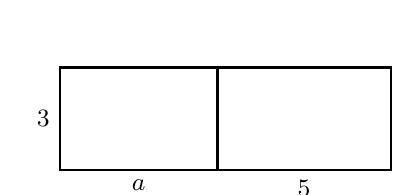
\begin{tikzpicture}[line width=0.8pt]
\draw (0,0) rectangle (2.0,1.3); \draw (2.0,0) rectangle (4.2,1.3);
\node[left,font=\small] at (0,0.65) {$3$};
\node[below,font=\small] at (1.0,0) {$a$};
\node[below,font=\small] at (3.1,0) {$5$};
\end{tikzpicture}}{Summe: & \underline{\hspace{4cm}} \\[8mm]
Produkt: & \underline{\hspace{4cm}}}
% terme-e4-k2-s8-v2
% pruef: 0.2*(30 + 15) == 9
\rs{Ein Rucksack kostet 30 €, eine Trinkflasche 15 €. Es gibt 20 \% Rabatt. Emre rechnet den Rabatt mit $0{,}2 \cdot 30 + 15$, Lea mit $0{,}2 \cdot (30 + 15)$. Welcher Term passt? Begründe und berechne den Rabatt.}{Lea; bei Emre fehlt $0{,}2$ vor der 15; Rabatt $9\,€$}
\end{nr}

% =================================================================== Einheit 4
\einheit{4}{Terme aufstellen und berechnen}
\merk{\mz{Vermindert um:}{„$x$ um 5 vermindert“: $\mathbf{x - 5}$}
\mz{Das Mehrfache einer Summe:}{„das Dreifache der Summe aus $x$ und 4“: $\mathbf{3 \cdot (x + 4)}$, mit Klammer}
\mz{Einsetzen:}{$3x^2$ für $x = -2$: $3 \cdot (-2)^2 = \mathbf{12}$}
\mz{Wichtig:}{Negative Zahlen in Klammern einsetzen; „5 vermindert um $x$“ ist $5 - x$, nicht $x - 5$.}}

\begin{nr}[b]{Berechne den Wert des Terms.}\label{nr:wert}
\begin{werte}
% terme-e1-k2-s1-v1 (vorgerechnet)
\rwv{4x - 3}{x = 5}{4 \cdot 5 - 3 = 17}
% terme-e1-k2-s1-v2
\rw{2x + 9}{x = -3}{3}
% terme-e1-k2-s1-v3
\rw{10 - 3x}{x = -2}{16}
% NEU
\rw{x^2 - 5x}{x = -2}{14}
% NEU
\rw{2x^2 + 3x}{x = -\frac{1}{2}}{-1}
% NEU
\rw{0{,}5a - 2b}{a = 8,\ b = -1{,}5}{7}
% NEU
\rw[GYM]{3 \cdot (x - y)^2 + xy}{x = 2,\ y = -1}{25}
\end{werte}
% terme-e2-k4-s11-v2
% pruef: 10*b - 5*b**2 - 7*b == 3*b - 5*b**2
% pruef: 3*2 - 5*2**2 == -14
\rs[P10 ’25]{Vereinfache den Term $10b - 5b^2 - 7b$ und berechne seinen Wert für $b = 2$.}{$3b - 5b^2$; für $b = 2$: $-14$}
\end{nr}

\begin{nr}[b]{Schreibe einen Term.}\label{nr:auf}
% terme-e1-k1-s2-v1
% pruef: 3*x + 8 == 3*x + 8
\rt{Das Dreifache einer Zahl $x$ wird um 8 vergrößert.}{$3x + 8$}
% terme-e1-k1-s2-v3
% pruef: 5*x + 1 == 5*x + 1
\rt{Das Fünffache einer Zahl $x$ wird um 1 vergrößert.}{$5x + 1$}
% GEÄNDERT terme-e1-k1-s3-v1 (Form: Feld neben der Figur)
% pruef: 5*x == 5*x
\rtx{Flächeninhalt des Rechtecks (Maße in cm):}{$5x$}
\figurfelder{\rechteck[seiten={5,x,,},punkte=]{3.2}{1.1}}{& \underline{\hspace{4cm}}}
% terme-e1-k1-s4-v2
% pruef: 2*e + 5*k == 2*e + 5*k
\rt{Eine Eintrittskarte kostet für Erwachsene $e$ Euro und für Kinder $k$ Euro. Es kommen 2 Erwachsene und 5 Kinder. Was zahlen alle zusammen?}{$2e + 5k$}
% terme-e1-k1-s5-v2
% pruef: m + 2*m + m + 5 == 4*m + 5
\rt{Tom hat $m$ Murmeln. Ina hat doppelt so viele wie Tom, Ali hat 5 mehr als Tom. Wie viele haben alle zusammen? Fasse zusammen.}{$4m + 5$}
% terme-e1-k1-s6-v1
% pruef: 2*(3*x + 2) == 6*x + 4
\rt{Verdreifache eine Zahl $x$, addiere 2 und verdopple die Summe.}{$2 \cdot (3x + 2)$}
% terme-e1-k1-s7-v3
\rtx[P10 ’17]{Das Sechsfache einer Zahl $x$ wird um zwei vermindert. Kreuze den passenden Term an.}{$6x - 2$}
\kreuzzeile{\kreuz{$6 \cdot (x - 2)$}\kreuz{$2 - 6x$}\kreuz{$6x - 2$}\kreuz{$6x - 2x$}}
% terme-e1-k1-s7-v2
\rtx[P10 ’23]{Die Summe aus dem Vierfachen einer Zahl $x$ und 9 wird halbiert. Kreuze den passenden Term an.}{$(4x + 9) : 2$}
\kreuzzeile{\kreuz{$4x + 9 : 2$}\kreuz{$(4x + 9) : 2$}\kreuz{$2 \cdot (4x + 9)$}\kreuz{$4x : 9 + 2$}}
\end{nr}

\begin{nr}{Abschluss}
% NEU
% pruef: 4*(x + 6) == 4*x + 24
\rt{Schreibe als Term: Die Summe aus einer Zahl $x$ und 6 wird vervierfacht.}{$4 \cdot (x + 6)$}
% terme-e1-k4-s4-v3
% pruef: 30 + 45*3 == 165
\rs{Ein Handwerker berechnet 30 € für die Anfahrt und 45 € je Arbeitsstunde. Stelle einen Term für die Rechnung in Euro bei $t$ Stunden auf. Was kostet ein Einsatz von 3 Stunden?}{$30 + 45t$; $165\,€$}
% terme-e1-k4-s2-v1
% pruef: 2*(3 + 5) == 16
% pruef: 2*3 + 5 == 11
\rs{Warum braucht man für „das Doppelte der Summe aus $x$ und 5“ eine Klammer? Begründe. Setze dazu $x = 3$ in $2 \cdot (x + 5)$ und in $2x + 5$ ein.}{$2 \cdot (3 + 5) = 16$, aber $2 \cdot 3 + 5 = 11$: ohne Klammer wird nur $x$ verdoppelt}
\end{nr}

% =================================================================== Zum Schluss
% Je Einheit eine Teilaufgabe mittlerer Höhe (a–e, gemischt), dann zwei
% höhere (f GYM wie Nr. kz, g P10 ’25 wie Nr. wert); Lösungen mit „falsch → Nr. n“.
\par\addvspace{10pt}
\begin{nr}{Zum Schluss}
\begin{kette}
% NEU (Einheit 2)
\falschk{\ref{nr:kz}}
\rk{3 \cdot (2a - 1) - (4a - 6)}{2a + 3}
% NEU (Einheit 1)
\falschk{\ref{nr:zus}}
\rk{5x + 2y - 7x + 4y - 3}{-2x + 6y - 3}
\end{kette}
\begin{werte}
% NEU (Einheit 4)
\falschk{\ref{nr:wert}}
\rw{4 - 3x^2}{x = -2}{-8}
\end{werte}
% NEU (Einheit 3)
% pruef: 5*y*(2*x - 3) == 10*x*y - 15*y
\falsch{\ref{nr:aus}}
\rt{Klammere aus: \ $10xy - 15y$}{$5y \cdot (2x - 3)$}
% NEU (Einheit 4)
% pruef: 15 + 3*x == 15 + 3*x
\falsch{\ref{nr:auf}}
\rt{Ein Schwimmbad verlangt 15 € Jahresbeitrag und 3 € je Besuch. Stelle einen Term für die Kosten in Euro bei $x$ Besuchen auf.}{$15 + 3x$}
\begin{kette}
% NEU (GYM, wie Nr. kz h)
\falschk{\ref{nr:pm}, \ref{nr:kz}}
\rk[GYM]{5a - \{\,2b - [\,3a - (b - a)\,]\,\}}{9a - 3b}
\end{kette}
% NEU (P10 ’25, wie Nr. wert h; Original 2025-GYM-B2a mit neuen Zahlen)
% pruef: 9*c - 4*c**2 - 6*c == 3*c - 4*c**2
% pruef: 3*(-1) - 4*(-1)**2 == -7
\falsch{\ref{nr:zus}, \ref{nr:wert}}
\rs[P10 ’25]{Vereinfache den Term $9c - 4c^2 - 6c$ und berechne seinen Wert für $c = -1$.}{$3c - 4c^2$; für $c = -1$: $-7$}
\end{nr}

% =================================================================== Lösungen
\clearpage
\noindent{\Large\bfseries Lösungen}\par\vspace{2pt}
\begin{multicols}{2}\raggedright\small\linespread{0.96}\selectfont
\mblsg
\end{multicols}
\end{document}
